\documentclass[11pt,a4paper]{article}
\usepackage[utf8]{inputenc}
\usepackage{amsmath}
\usepackage{amsfonts}
\usepackage{amssymb}
\usepackage[utf8]{inputenc}
\usepackage[T1]{fontenc}
\usepackage{textcomp}
\usepackage{gensymb}
\usepackage{graphicx}
\begin{document}

\section*{Response test}

This test renders a graph for $\theta_r$, $\phi_r$. For each $\theta_r$ an integration is performed for an incident direction $\omega_i$ around a sphere. Using this integration it can be shown for a specific position, in what directions the response is spread. So, light can enter from any direction after an arbitrary sequence of scattering events. That is why the integration is performed around the sphere). We are interested in specific points inside and outside of the model. What we expect to see is that for points inside the model, the light is more widely spread due to the scattering events, compared to points outside the model.\\

The hair model looks as follows:

\begin{figure}[h]
\begin{center}
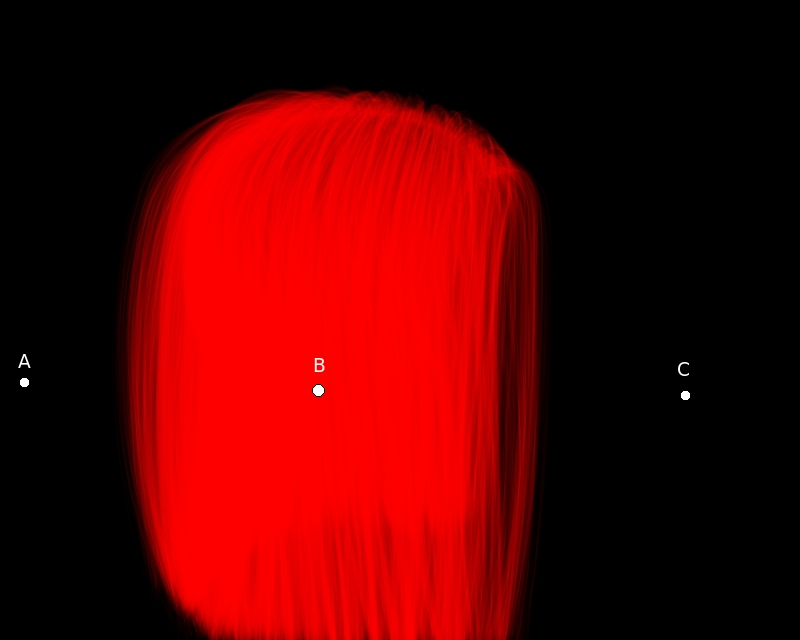
\includegraphics[scale=0.5]{hairmodel.jpg}
\caption{Plot of the hair model with indications for positions A, B and C. A sphere is placed to the left of the model that is acting as area light.}
\end{center}
\end{figure}

The light source is placed to the left of the hair model at position (-8, 3, 0). 
The hair model is placed at the origin of the scene and translated 2 units upwards. The dimensions of the hair model are approximately 2.1 by 2.1 for the width (x-axis) and depth (z-axis) and 4.38 tall. Three different positions are used to generate a response graph. Position A is situated to the left of the hair model at position (-3, 2, 0). Position B is placed in the center of the model at (0, 2, 0) and position C is placed to the right of the model at (3, 2, 0).

We want to render a 2D slice, showing how the light from the light source is spread. At this moment the graph is shown as a spherical plot (a $\theta$ and $\phi$ axis). The $\phi$ direction is held constant, because the integration is performed for $\theta_r$ only.

\begin{figure}
\begin{center}
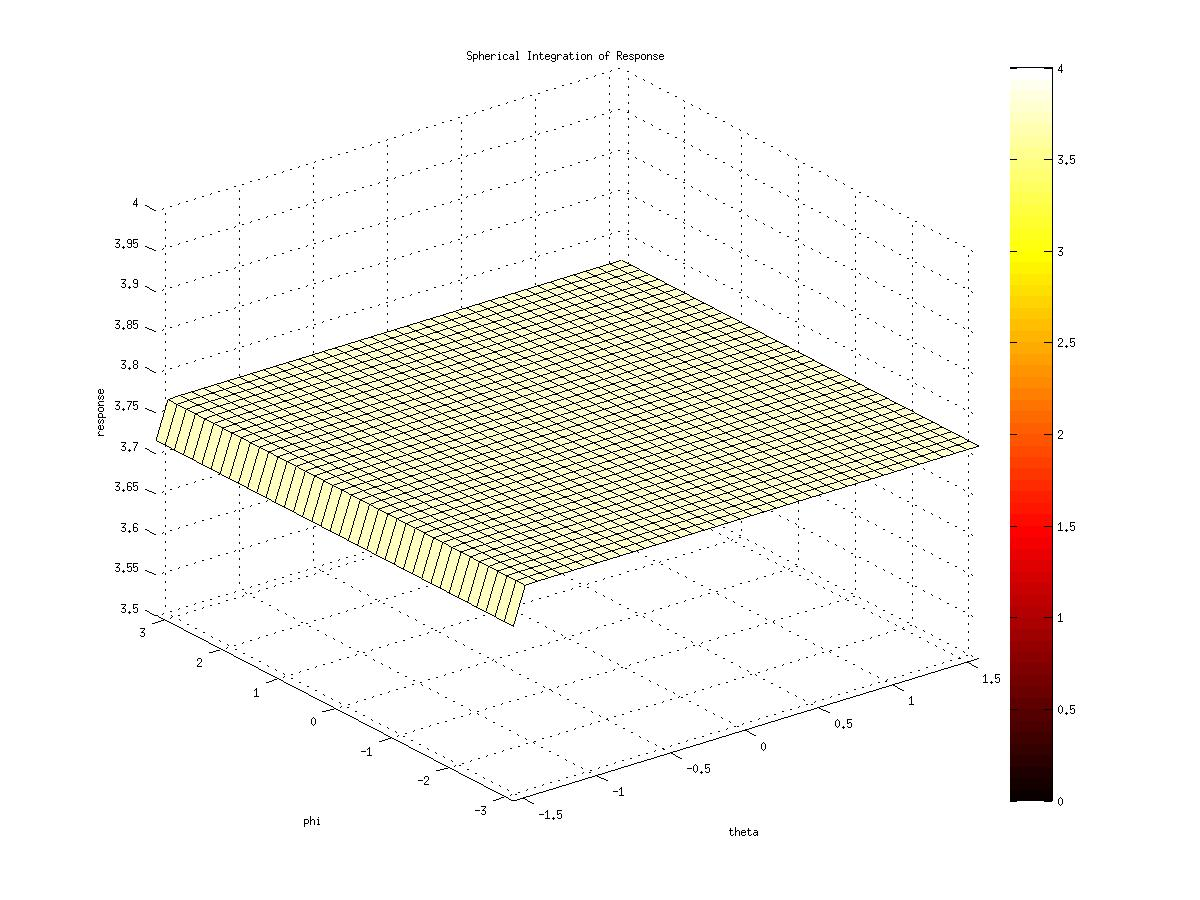
\includegraphics[scale=0.3]{outputA.jpg}
\caption{Plot for position A: (-3, 2, 0). Position A is placed to the left of the hair model in between the area light (a sphere) and the hair model.}
\end{center}
\end{figure}

\begin{figure}
\begin{center}
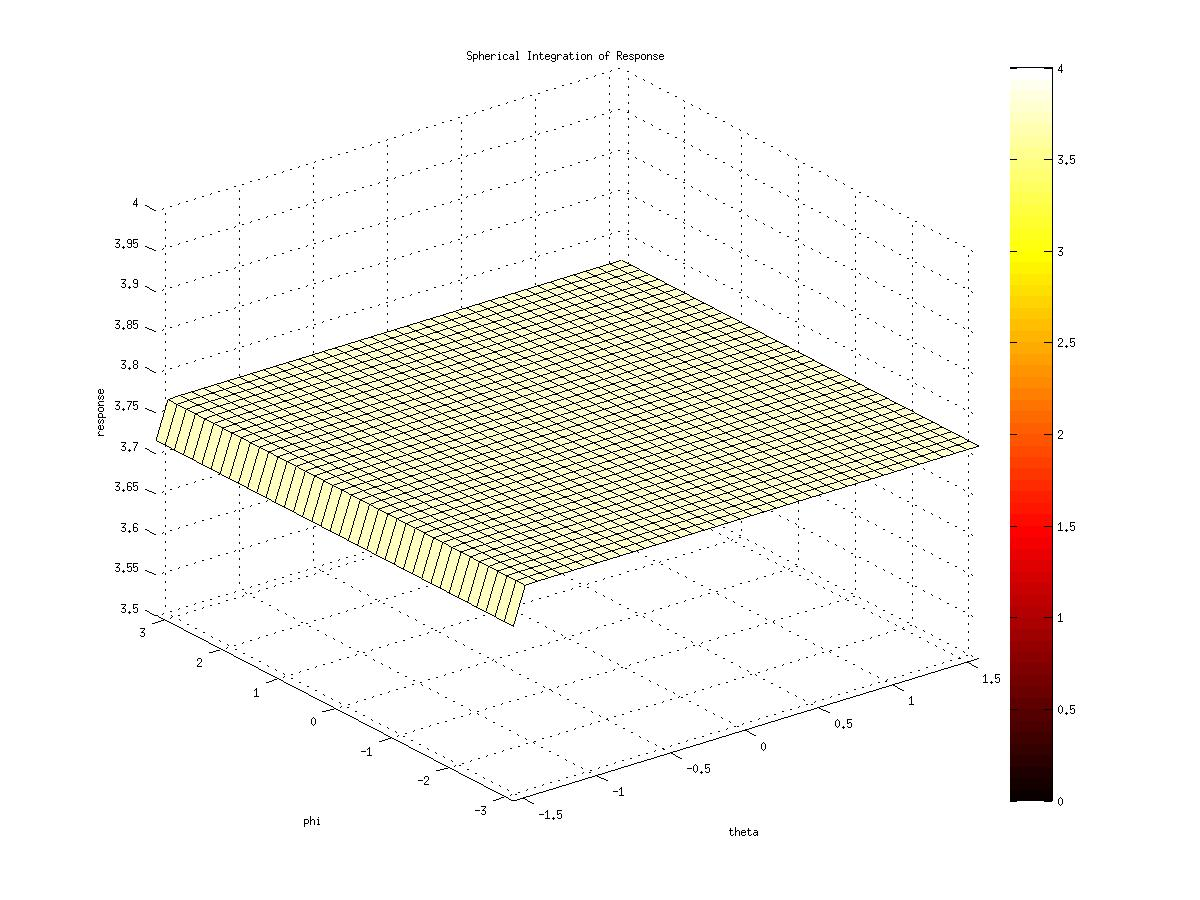
\includegraphics[scale=0.3]{outputB.jpg}
\caption{Plot for position B: (0, 2, 0). Position B is placed in the center of the hair model.}
\end{center}
\end{figure}

\begin{figure}
\begin{center}
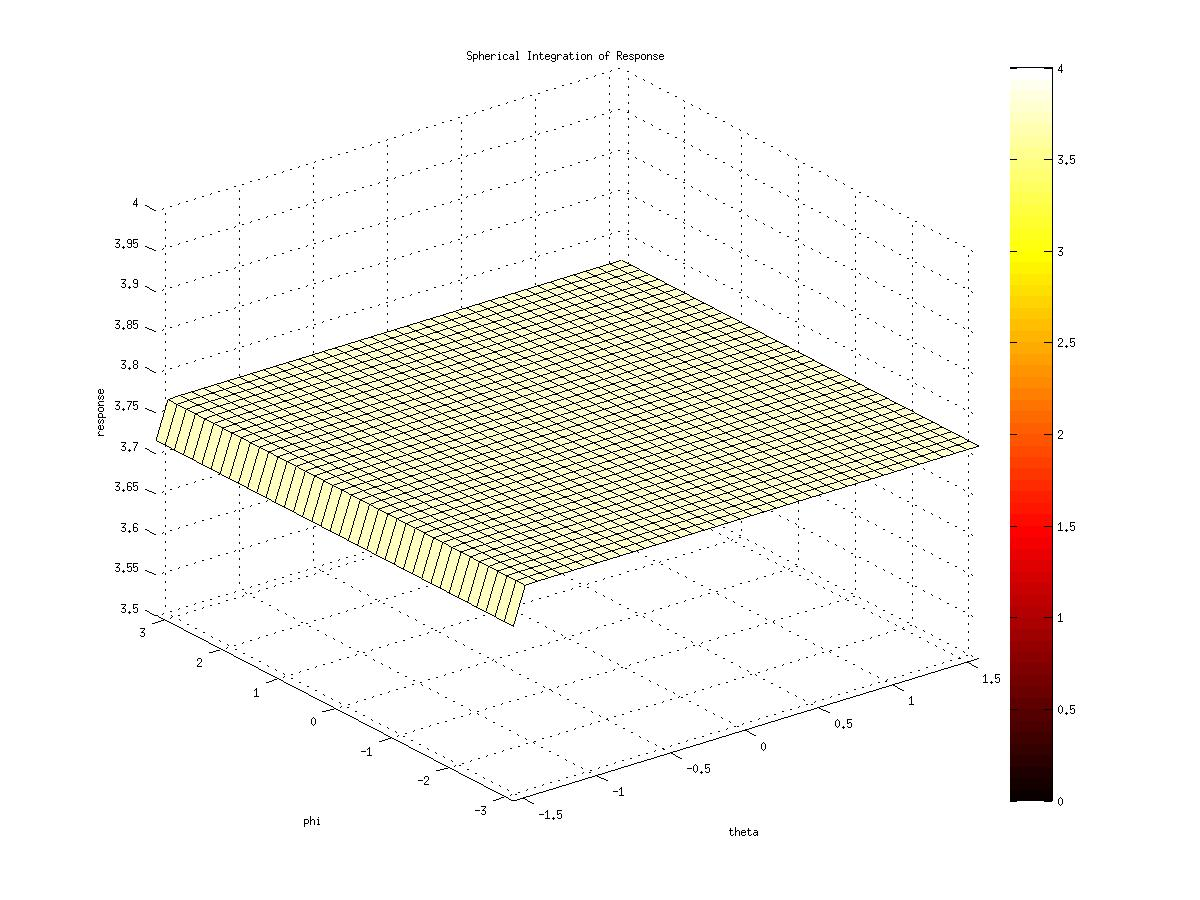
\includegraphics[scale=0.3]{outputC.jpg}
\caption{Plot for position C: (3, 2, 0). Position C is placed to the right of the hair model. The hair model obscures a direct visual on the area light source (a sphere) as seen from position C.}
\end{center}
\end{figure}


As can be seen from the plots, it looks different from what we expect. They all look similar and there is hardly any variation along the $\theta$ axis. Integration around a sphere might reduce the impact of the spikes, leading to a more general response. It is also weird that position A, that is outside of the model, shows the same amount of response to the direction of the light source, while the light has not yet undergone any scattering events.

\end{document}

